%% 
%% Copyright 2007-2026 Elsevier Ltd
%% 
%% This file is part of the 'Elsarticle Bundle'.
%%
\documentclass[preprint,12pt]{elsarticle}

%% The amssymb package provides various useful mathematical symbols
\usepackage{amssymb}
%% The amsmath package provides various useful equation environments.
\usepackage{amsmath}

%% Additional packages
\usepackage{booktabs}
\usepackage{hyperref}

\usepackage{float}
%% Math operators
\DeclareMathOperator*{\argmin}{argmin}

\journal{Neurocomputing}

\begin{document}

\begin{frontmatter}

%% Title
\title{Learning algorithm shapes attractor dynamics: comparing reinforcement 
and supervised learning in decision-making RNNs}

%% Authors
\author[iapras,lobachevsky]{Roman A. Kononov}
\author[iapras,msu]{Nikita A. Pospelov}
\author[msu]{Konstantin V. Anokhin}
\author[iapras,lobachevsky]{Vladimir V. Nekorkin}
\author[iapras,lobachevsky]{Oleg V. Maslennikov\corref{cor1}}
\ead{olmaov@ipfran.ru}

\cortext[cor1]{Corresponding author}

%% Affiliations
\affiliation[iapras]{organization={Institute of Applied Physics of the Russian Academy of Sciences},
            addressline={46 Ulyanov Street}, 
            city={Nizhny Novgorod},
            postcode={603950}, 
            country={Russia}}

\affiliation[msu]{organization={Institute for Advanced Brain Studies, Lomonosov Moscow State University},
            addressline={1 Leninskie Gory}, 
            city={Moscow},
            postcode={119991}, 
            country={Russia}}

\affiliation[lobachevsky]{organization={Radiophysics Faculty, Lobachevsky University},
            addressline={23 Gagarin Avenue}, 
            city={Nizhny Novgorod},
            postcode={603022}, 
            country={Russia}}

%% Abstract
\begin{abstract}
We introduce a multi-scale analytical framework for characterizing how the choice of learning algorithm shapes the computational solutions discovered by recurrent neural networks (RNNs). Combining dynamical systems theory, information-theoretic measures, and population-level analysis, we systematically compare RNNs trained via reinforcement learning (RL) and supervised learning (SL) on context-dependent decision-making tasks. Our framework reveals that these learning paradigms produce qualitatively different internal dynamics despite achieving comparable task accuracy. Through dynamical systems analysis, we show that RL-trained networks develop hybrid attractor architectures combining stable fixed-point attractors for decision maintenance with quasi-periodic attractors for stimulus encoding, whereas SL-trained networks converge predominantly to fixed-point-only solutions. At the population level, RL produces functionally balanced neural ensembles with approximately equal sizes for opposing stimulus representations, while SL yields more heterogeneous structures. We demonstrate that the prevalence of quasi-periodic dynamics in RL networks is modulated by weight initialization and correlates with the encoding of ambiguous stimuli. Our results establish that behavioral equivalence does not imply mechanistic equivalence, and demonstrate the utility of comprehensive dynamical analysis for understanding learning-algorithm-dependent computation in neural networks. The proposed framework provides a systematic methodology applicable to future investigations across diverse task domains and offers insights relevant to both computational neuroscience and the design of adaptive AI systems.
\end{abstract}

%%Research highlights
\begin{highlights}
\item Multi-scale framework integrates dynamical systems, information theory, and population analysis
\item RL produces hybrid attractor architectures; SL converges to fixed-point-only solutions
\item RL yields balanced neural populations; SL produces heterogeneous structures
\item Behavioral equivalence does not imply mechanistic equivalence between learning paradigms
\item Framework provides systematic methodology for comparing learning algorithms
\end{highlights}

%% Keywords
\begin{keyword}
recurrent neural networks \sep reinforcement learning \sep attractor dynamics \sep decision-making \sep dynamical systems \sep neural population coding
\end{keyword}

\end{frontmatter}


%==============================================================================
\section{Introduction}
\label{sec:introduction}
%==============================================================================

Developing artificial intelligence capable of the flexible, context-dependent decision-making seen in biological systems remains a significant challenge in machine intelligence \cite{botvinick2020deep}. Recurrent neural networks (RNNs) have become central to this pursuit, serving as powerful models for emulating cognitive computations \cite{vyas2020computation, barak2017recurrent} and revealing the relationship between network structure and emergent function \cite{durstewitz2023reconstructing}. A key principle underlying both biological and artificial cognition is the use of attractor dynamics, where neural activity settles into stable patterns---such as fixed points for memory maintenance or limit cycles for rhythmic processes---to implement computation \cite{fiete2022attractor, wang2001dynamics}. Recent work has shown that RNNs trained with reinforcement learning (RL) can spontaneously self-organize low-dimensional representations that mirror the functional architecture of the primate brain, establishing attractor dynamics as a convergent strategy for intelligent behaviour \cite{bellafard2024volatile, wang2024working}.

However, a critical gap separates the analysis of fully trained networks from a true understanding of their computational capabilities: we lack a mechanistic account of how these sophisticated computational structures emerge during the learning process itself. This gap is especially acute for reinforcement learning. While RL's trial-and-error exploration embodies biological learning principles more closely than supervised learning, it remains far less understood from a dynamical systems perspective \cite{song2017reward}. While we know that trained networks employ low-dimensional manifolds \cite{ganguli2023low} and exhibit mixed selectivity \cite{rigotti2013importance}, it remains unclear how the learning algorithm itself---the choice between reward-driven exploration (RL) and explicit error correction (SL)---fundamentally dictates the type of computational solutions that are discovered.

\textbf{Methodological gap.} While previous studies have analyzed trained networks post-hoc using various dynamical systems tools, there is no established integrative framework for systematically comparing how different learning algorithms shape internal dynamics. Existing approaches typically focus on single aspects---either attractor classification, or population analysis, or information encoding---without combining these perspectives to obtain a comprehensive picture of learning-dependent computational structure. Previous work has characterized the outcomes of learning---the attractor landscapes and population codes of trained networks \cite{sussillo2013opening, ganguli2023low}---but not the learning process itself as a computational discovery mechanism. Yet RL's reward-driven exploration and SL's explicit gradient descent represent fundamentally different optimization processes that may impose distinct constraints on the space of discoverable solutions. Without direct comparison under controlled conditions, we cannot determine whether these learning paradigms are merely alternative routes to similar solutions or gateways to fundamentally different computational strategies.

Here we establish a framework for understanding how learning algorithms sculpt neural computation. We systematically compare RNNs trained via reinforcement learning and supervised learning on identical context-dependent decision-making tasks \cite{mante2013context}, tracking the emergence of computational solutions from random initialization to expert performance. By analyzing networks throughout training using dynamical systems theory, information theory, and population-level analysis, we reveal how the learning paradigm itself determines the computational strategies that emerge. Our approach integrates three complementary levels of analysis: (1) dynamical systems characterization of attractor types and stability via eigenvalue analysis, (2) information-theoretic quantification of neural selectivity using mutual information, and (3) population-level analysis of functional organization through template matching. The primary contribution of this work is methodological---we demonstrate how this integrated framework reveals systematic differences between learning paradigms that would not be apparent from behavioral performance metrics alone.

We deliberately chose depth over breadth: rather than surveying many tasks superficially, we performed exhaustive dynamical characterization of a single well-understood paradigm. This approach reveals algorithmic signatures that would be invisible in behavioral comparisons alone, establishing a template for future multi-task investigations. The extension to other task types, including multi-choice decisions and continuous-variable tasks with different attractor geometries (e.g., ring attractors), remains an important direction for future work.

We discover that RL and SL converge on fundamentally different computational solutions, despite solving identical tasks. RL spontaneously discovers hybrid attractor architectures that balance stable fixed-point attractors for decision maintenance with quasi-periodic (oscillatory) attractors for flexible evidence integration. This dynamical richness stands in stark contrast to SL, which overwhelmingly converges on simpler, fixed-point-only solutions. This divergence is mirrored at the population level: RL sculpts functionally balanced neural populations through implicit regularization \cite{turner2023implicit}, while SL produces more heterogeneous and specialized ensembles. The emergence of quasi-periodic dynamics in RL-trained networks correlates with performance and is controllably modulated by weight initialization.

By elucidating the evolutionary trajectory of these neural computations, our work provides a bridge between the learning rule and the learned algorithm. These findings offer mechanistic insights into how biological circuits may self-organize through reward-driven plasticity \cite{williams1998dopamine, bermudez2021deep} and provide principles relevant to designing AI systems that can learn flexible and robust behaviors through autonomous interaction with their environment \cite{stroud2024computational, hennig2023emergence}.


%==============================================================================
\section{Methods}
\label{sec:methods}
%==============================================================================

\subsection{RNN model and task specification}
\label{subsec:model}

All numerical experiments utilized a vanilla recurrent neural network (RNN) defined by the state update equation:
\begin{equation}
\mathbf{h}_{t+1} = \text{ReLU}(\mathbf{W}_{hh} \mathbf{h}_t + \mathbf{W}_{ih} \mathbf{I}_t),
\label{eq:RNN}
\end{equation}
where $\mathbf{h}_t \in \mathbb{R}^{N_{hidden}}$ is the hidden state vector at time $t$ with $N_{hidden} = 250$. This network size was chosen to be consistent with similar studies of RNNs on cognitive tasks. This size is sufficiently large to allow for the emergence of complex dynamics and population structures, yet small enough to remain computationally tractable for training large ensembles of networks. $\mathbf{I}_t \in \mathbb{R}^{N_{input}}$ is the input vector ($N_{input} = 7$), $\mathbf{W}_{hh}$ is the recurrent weight matrix, and $\mathbf{W}_{ih}$ is the input weight matrix. The agent's action policy is derived from the hidden state via a linear readout $\mathbf{o}_{t} = \mathbf{W}_{ho} \mathbf{h}_t$, followed by a softmax function to produce action probabilities over three actions (fixation, choice 1, choice 2).

The input vector $\mathbf{I}_t$ for each trial was composed of a noise-free signal $\mathbf{I}^{pure}$ and an additive noise term:
\begin{equation}
\mathbf{I}_t = \mathbf{I}^{pure}_t + \alpha \mathbf{r}_t,
\label{eq:input}
\end{equation}
where $\mathbf{r}_t$ is a random vector with components drawn from $\mathcal{U}(-1,1)$ and $\alpha = 0.1$. The noise-free input $\mathbf{I}^{pure}$ encodes seven task variables: a fixation signal $(F)$, two pairs of stimulus inputs corresponding to the two contexts ($A_1$, $A_2$ and $B_1$, $B_2$), and two context cues ($C_A$, $C_B$). Stimulus coherence for each context was defined as:
$$coh_A = A_1 - A_2, \quad coh_B = B_1 - B_2,$$
sampled uniformly from $[-1, 1]$.

The trial structure consisted of four stages: fixation (10 time steps), stimulus presentation (20 time steps), delay (10 time steps), and decision (1 time step). Network weights were initialized from a uniform distribution: recurrent and input weight matrices from $\mathcal{U}(-\delta, \delta)$, and readout weights from $\mathcal{U}(-0.1, 0.1)$. We systematically varied the initialization width $\delta \in \{0.05, 0.1, 0.15, 0.2, 0.25, 0.3\}$ across experiments to examine its effect on emergent dynamics.


\subsection{Training procedures}
\label{subsec:training}

We trained four ensembles of networks across two tasks (simple decision-making DM and context-dependent decision-making CtxDM) and two learning paradigms. For each condition, we trained 50 networks with different random seeds. Training was terminated when a network achieved 95\% accuracy on a held-out validation set of 1000 trials, or after a maximum of 500,000 training iterations. 
Training success rates varied with initialization width 
(see Appendix~\ref{app:additional}, Fig.~\ref{fig:S5}).


\subsubsection{Reinforcement learning}
Networks were trained using the Proximal Policy Optimization (PPO) algorithm \cite{schulman2017proximal}, an actor-critic method implemented in Stable-Baselines3. The reward structure was: $+1$ for correct choice, $-1$ for incorrect choice, $-0.1$ for breaking fixation (choosing during fixation/delay periods), and $0$ otherwise. Hyperparameters were set according to Table~\ref{tab:hyper} to ensure stable learning.

\subsubsection{Supervised learning}
Supervised baselines were trained using the Adam optimization algorithm with a cross-entropy loss function. The target was ``fixation'' for all timesteps except the final decision step, where the target was the correct choice based on the context-relevant coherence sign. See Table~\ref{tab:hyper} for hyperparameters.

\begin{table}[H]
\centering
\caption{Hyperparameter configuration for reinforcement and supervised learning algorithms.}
\label{tab:hyper}
\begin{tabular}{lcclc}
\toprule
\multicolumn{2}{c}{\textbf{PPO (RL)}} & & \multicolumn{2}{c}{\textbf{Adam (SL)}} \\
\cmidrule{1-2} \cmidrule{4-5}
Parameter & Value & & Parameter & Value \\
\midrule
$\gamma$ (discount) & 0.99 & & $\beta_1$ & 0.9 \\
$\lambda_{gae}$ & 0.95 & & $\beta_2$ & 0.999 \\
$\epsilon$ (clip) & 0.2 & & learning rate & 0.0003 \\
entropy coef. & 0 & & max grad norm & 0.5 \\
value func. coef. & 0.5 & & batch size & 64 \\
learning rate & 0.0003 & & & \\
batch size & 64 & & & \\
\bottomrule
\end{tabular}
\end{table}

\subsubsection{Computational details}
All simulations were performed using Python 3.9, PyTorch 1.12, and Stable-Baselines3 1.6. Training was performed on NVIDIA RTX 3090 GPUs (approximately 2000 GPU-hours total). Ensemble sizes and weight initialization widths ($\delta$) varied by experiment as detailed in the Results.


\subsection{Dynamical systems analysis}
\label{subsec:dynamical}

\subsubsection{Attractor identification and classification}
To identify attractors, we extended the duration of the stimulus stage to 1000 time steps and allowed the system dynamics to converge to a stationary state. For ReLU networks, the dynamics within a given activation pattern (set of active neurons) are piecewise linear. For a given set of active neurons indexed by $\mathcal{A}$, the dynamics are governed by:
\begin{equation}
\mathbf{h}^{\mathcal{A}}_{t+1} = \mathbf{W}^{\mathcal{A}}_{hh} \mathbf{h}^{\mathcal{A}}_t + \mathbf{s}^{\mathcal{A}},
\label{eq:linear}
\end{equation}
where $\mathbf{W}^{\mathcal{A}}_{hh}$ is the submatrix of recurrent weights for active neurons and $\mathbf{s}^{\mathcal{A}}$ is the effective input.

An attractor was classified based on the eigenvalues of $\mathbf{W}^{\mathcal{A}}_{hh}$:
\begin{itemize}
    \item \textbf{Stable fixed point}: The leading eigenvalue $\mu_{lead}$ satisfies $|\mu_{lead}| < 1$.
    \item \textbf{Quasi-periodic attractor}: A complex conjugate eigenvalue pair $\mu_{con}$ satisfies $|\mu_{con}| > 1$ while the system remains bounded (verified by simulation).
\end{itemize}

For each network, we computed attractor types across a $44 \times 44$ grid of coherence values for both contexts, yielding 3872 attractor classifications per network.


\subsubsection{Population classification}
We classified neurons into functional groups using a template-matching procedure based on their complete response profiles across the coherence space. This objective method provides a robust definition of functional specialization.

First, for each neuron $n$, we constructed an activity-type matrix $\mathbf{M}^{(n)}$ over the coherence grid. For each point in this grid, we determined the neuron's participation in the stationary dynamics for each of the two possible contexts (Context $A$ and Context $B$). Based on this, we assigned one of four integer labels to the corresponding entry:
\begin{itemize}
\item 0 ($U_s$): The neuron is silent (does not participate) in the stationary dynamics for either context.
\item 1 ($U_A$): The neuron participates exclusively in the dynamics for Context A.
\item 2 ($U_B$): The neuron participates exclusively in the dynamics for Context B.
\item 3 ($U_a$): The neuron participates in the dynamics for both contexts.
\end{itemize}

Second, we defined four idealized template matrices $\mathbf{M}^c$ for $c \in \{\mathrm{G}_s, \mathrm{G}_+, \mathrm{G}_-, \mathrm{G}_a\}$ representing the canonical activity-type profiles for the populations that consistently emerged in trained networks (Fig.~\ref{fig:evo_labs}). Finally, each neuron was assigned to the population $c$ whose template $\mathbf{M}^c$ minimized the squared error with its observed activity-type matrix:
\begin{equation}
c^* = \argmin_{c \in \{\mathrm{G}_s,\mathrm{G}_+,\mathrm{G}_-,\mathrm{G}_a\}} \sum_{i,j} (M^{(n)}_{i,j}-M^{c}_{i,j})^2.
\label{eq:population}
\end{equation}


\subsection{Information-theoretic analysis}
\label{subsec:information}

Neuronal selectivity was quantified using Mutual Information (MI) between single-neuron activity and task variables. We used the computationally efficient Gaussian Copula Mutual Information (GCMI) method \cite{gcmi2016statistical}. MI was computed between firing rate (averaged over 5 time-step windows) and the binary variable indicating sign of primary coherence. Statistical significance was assessed through permutation testing: for each neuron, we generated a null distribution from 10,000 temporally shuffled surrogates and compared the observed MI against this distribution. Multiple comparisons were controlled using Holm's sequential procedure with family-wise error rate $\alpha = 0.01$.


\subsection{Dimensionality reduction and visualization}
\label{subsec:dimensionality}

To visualize high-dimensional neural trajectories, we trained a three-layer autoencoder with a bottleneck size of $N_{code}=3$. The architecture consisted of encoder ($N_{hidden} \rightarrow 128 \rightarrow N_{code}$) and decoder ($N_{code} \rightarrow 128 \rightarrow N_{hidden}$), with ReLU activations in hidden layers. To ensure interpretable and consistent visualizations across training epochs, we added an alignment term to the standard $L_2$ reconstruction loss:
\begin{equation}
\mathcal{L} = ||\mathbf{h} - \hat{\mathbf{h}}||_2^2 + \lambda \mathcal{L}_{align},
\label{eq:autoencoder}
\end{equation}
where $\mathcal{L}_{align} = - (R(C_1, coh_{prim}) + R(C_2, coh_{sec}))$, with $R$ being the Pearson correlation coefficient, $C_{1,2}$ being the first two latent dimensions, and $\lambda=0.1$. This alignment term encourages the primary axes of the latent space to consistently correspond to the primary task variables, enabling meaningful comparison of state-space geometry across different stages of training. Autoencoders were trained separately for each network snapshot using Adam optimizer (learning rate 0.001) for 1000 epochs on hidden state data from 500 trials.


%==============================================================================
\section{Results}
\label{sec:results}
%==============================================================================

\subsection{Overview of the analytical framework}
\label{subsec:overview}

Our framework integrates three complementary analytical approaches (Fig.~\ref{fig:scheme}): (1) eigenvalue-based attractor classification to characterize the dynamical landscape, (2) template-matching population analysis to identify functional neural groups, and (3) mutual information analysis to validate functional roles. We applied this framework to compare RL and SL-trained networks on context-dependent decision-making.

Both RL and SL networks achieved high task accuracy (>95\%), demonstrating that both paradigms successfully solve the task. However, as we show below, the internal computational strategies differ substantially.


\begin{figure}[!htbp]
\centering
\includegraphics[width=\textwidth]{Figure_1_NormilizeLabelLetters.pdf}
\caption{\textbf{Task structure and emergent architecture of a recurrent neural network trained with reinforcement learning.}
(a) Temporal structure of a single trial, showing the distinct fixation, stimulus, delay, and decision stages.
(b) Schematic of the vanilla RNN architecture with $N_{hidden}$ units.
(c) Time-resolved output probabilities from a trained network, illustrating the formation of a decision.
(d) The first principal component of hidden layer activity, capturing the dominant dynamical mode during a trial.
(e) The network's decision boundary in the two-dimensional coherence space, demonstrating successful context-dependent choices.
(f) Raster plot of the full hidden layer activity, revealing complex population-level dynamics.
(g) Recurrent weight matrix of the trained network, reorganized according to functionally distinct neural populations identified in our analysis. The structured connectivity, featuring strong intra-population excitation and inter-population inhibition, was not pre-specified but emerged entirely through reward-driven learning.}
\label{fig:scheme}
\end{figure}


\subsection{RL and SL produce different attractor types}
\label{subsec:attractors}

To investigate how learning rules shape neural computation, we trained recurrent neural networks (RNNs) on a context-dependent decision-making (CtxDM) task, a canonical benchmark for cognitive flexibility \cite{mante2013context}. In this task, an agent must integrate one of two noisy stimulus streams while ignoring the other, based on a contextual cue. The task unfolds across distinct trial stages---fixation, stimulus presentation, delay, and decision---requiring the network to maintain and manipulate information over time (Fig.~\ref{fig:scheme}a-c). The vanilla RNN architecture, featuring ReLU nonlinearities, was trained using two distinct paradigms: reward-driven Proximal Policy Optimization (PPO), a standard reinforcement learning (RL) algorithm, and gradient-based Adam optimization with a cross-entropy loss, a supervised learning (SL) approach.

While networks trained under both paradigms can achieve high task accuracy (Fig.~\ref{fig:scheme}e), analysis of their internal dynamics reveals that they converge on different computational strategies. These emergent strategies are reflected in the complex, population-level activity patterns (Fig.~\ref{fig:scheme}d,f) and the highly structured recurrent connectivity that develops during training (Fig.~\ref{fig:scheme}g). We systematically characterized the attractor landscape of trained networks by analyzing the stationary dynamics during prolonged stimulus presentation. This revealed two primary classes of solutions for stimulus encoding: stable fixed points, where neural activity converges to a single static pattern, and quasi-periodic attractors, where activity settles into a persistent, rhythmic oscillation. Attractor classification was validated via eigenvalue analysis (Appendix~\ref{app:validation}, Fig.~\ref{fig:S6}).


The choice between these encoding mechanisms represents a foundational difference between the learning paradigms. As shown across large ensembles of networks, RL consistently discovers solutions rich in quasi-periodic dynamics, particularly for ambiguous, low-coherence stimuli. In stark contrast, SL overwhelmingly favors simpler, fixed-point attractors across the entire stimulus space (Fig.~\ref{fig:third}a-d). This divergence suggests that the exploratory nature of RL uncovers a broader and more complex solution space than the explicit error-correction of SL \cite{zhang2021geometric}.


\begin{figure}[!htbp]
\centering
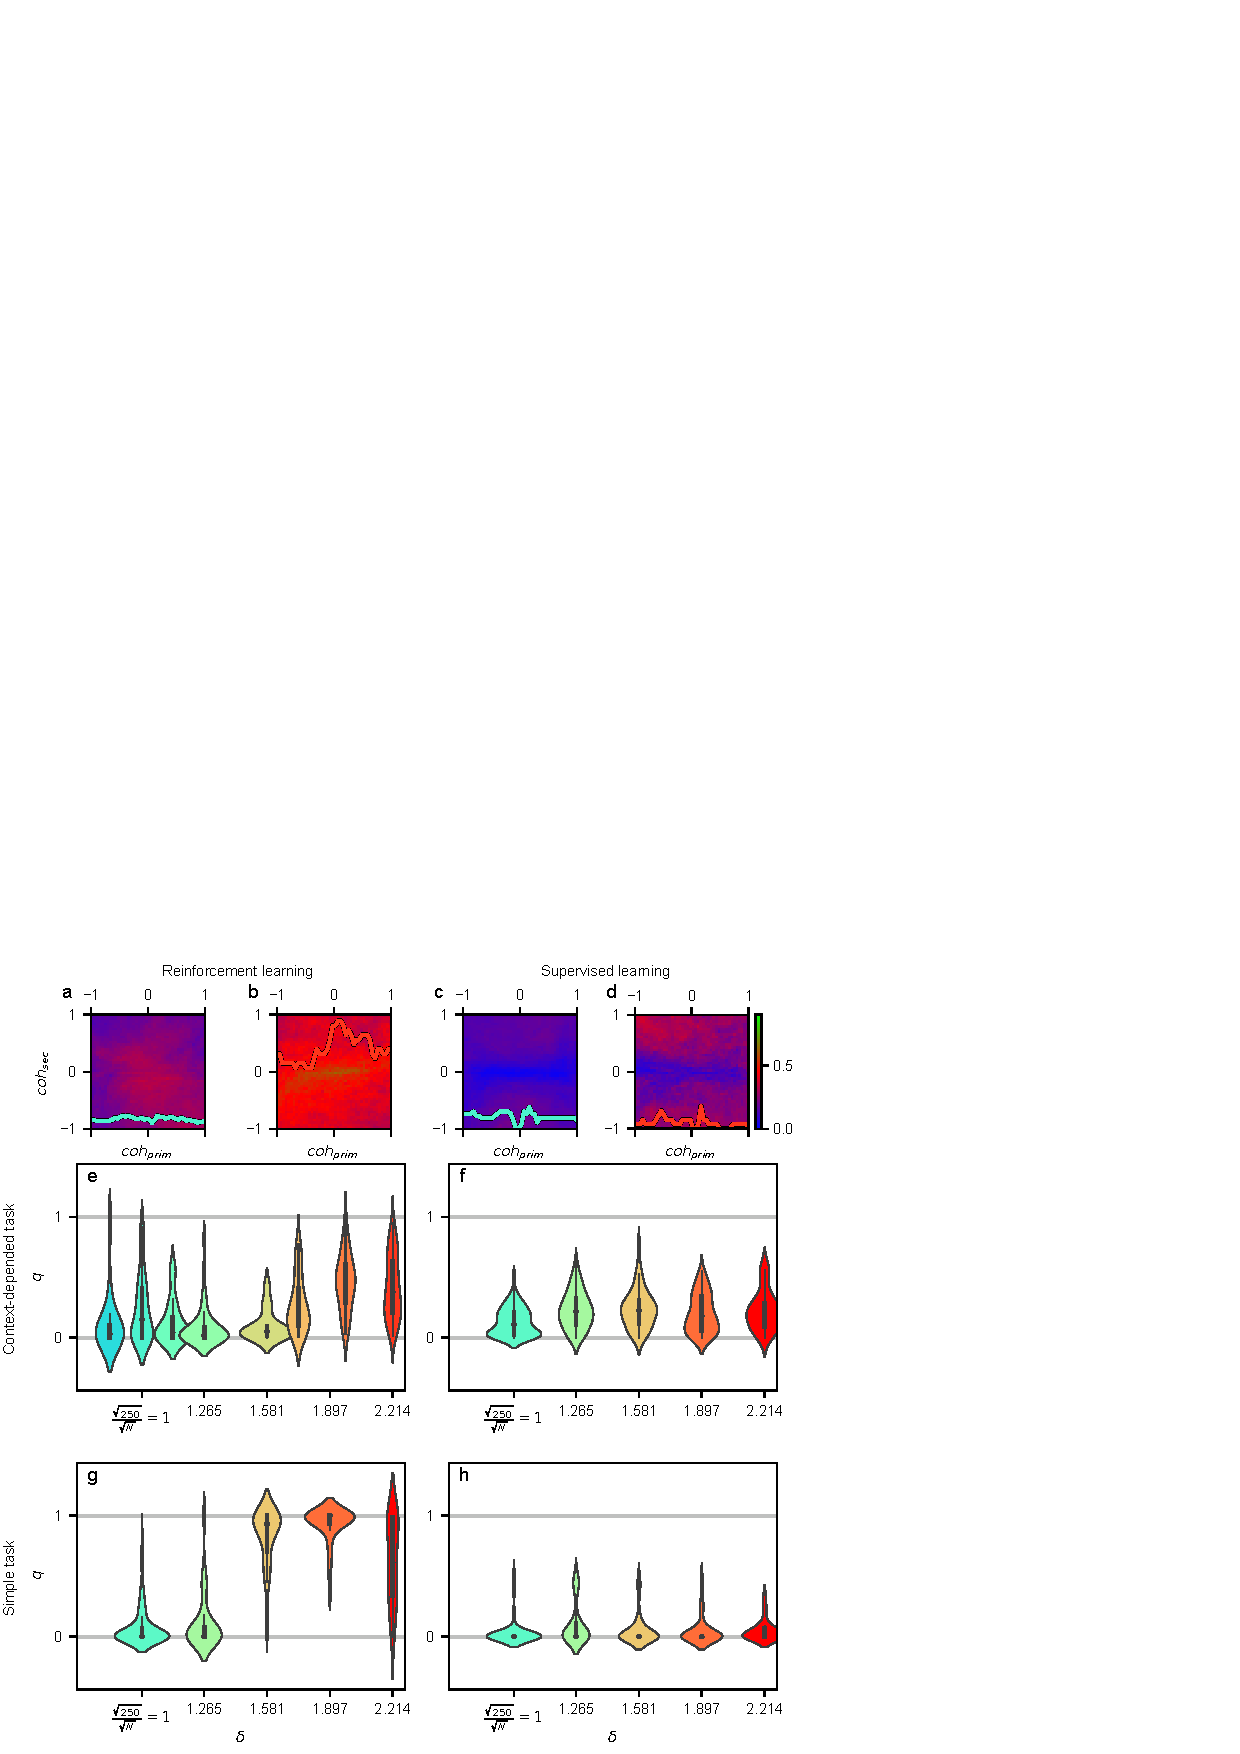
\includegraphics[width=0.95\textwidth]{Figure5.pdf}
\caption{\textbf{Comparison of attractor types between RL and SL.}
(a--d) Probability of a stimulus-encoding attractor being quasi-periodic (oscillatory) across the coherence parameter space. The learning algorithm fundamentally alters the solution type: reinforcement learning (a, b) consistently finds oscillatory solutions, particularly for ambiguous, low-coherence stimuli, while supervised learning (c, d) overwhelmingly converges to stable fixed points. This divergence is amplified by broader weight initializations (b, d). Panels (a, c): $\delta=0.1$; (b, d): $\delta=0.3$. Color scale: 0 (blue, fixed-point) to 1 (red, quasi-periodic).
(e--h) Aggregated statistics confirm the prevalence of quasi-periodic attractors is significantly higher in RL than SL across all initialization widths ($\delta$) and for both context-dependent (CtxDM; e, f) and simple (DM; g, h) tasks.}
\label{fig:third}
\end{figure}


The total fraction of quasi-periodic attractors is significantly higher in RL-trained networks across all conditions (Fig.~\ref{fig:third}e-h). Furthermore, this effect is powerfully modulated by the initial weight distribution, a critical hyperparameter in network training. Broader initial weight distributions (a larger half-width $\delta$) dramatically amplify the prevalence of oscillatory dynamics in RL networks, while having a negligible effect on SL networks. This sensitivity to initialization suggests that RL's reward-driven exploration is adept at harnessing initial dynamical richness, whereas SL's supervised gradient descent actively prunes such complexity in favor of the simplest stable solutions \cite{sussillo2013opening}.

We also examined a simpler decision-making task (DM) without context-dependence. The same qualitative pattern was observed: RL produced more quasi-periodic solutions than SL (Fig.~\ref{fig:third}g-h), indicating that this difference is not specific to the context-dependent task structure.

Table~\ref{tab:comparison} summarizes the quantitative differences between RL and SL solutions observed in our experiments.


\begin{table}[!htbp]
\centering
\caption{Summary comparison of RL and SL network properties observed in this study.}
\label{tab:comparison}
\begin{tabular}{lcc}
\toprule
\textbf{Property} & \textbf{RL} & \textbf{SL} \\
\midrule
Quasi-periodic attractor prevalence & 30--60\% & $<$10\% \\
Population balance ($|\mathrm{G}_+|/|\mathrm{G}_-|$) & $\approx$1.0 & 0.5--2.0 (variable) \\
Sensitivity to initialization ($\delta$) & High & Low \\
Final task accuracy & $\approx$95\% & $\approx$95\% \\
\bottomrule
\end{tabular}
\end{table}


\subsection{Hybrid attractor architecture in RL networks}
\label{subsec:hybrid}

The richer dynamics discovered through RL are not arbitrary but are organized into a sophisticated hybrid computational architecture that separates stimulus encoding from decision-making. By visualizing the high-dimensional neural trajectories in a low-dimensional space learned by an autoencoder, we can observe the formation of this architecture throughout training (Fig.~\ref{fig:AE}).

In the fully trained network, distinct computational functions are mapped onto geometrically distinct regions of the state space. Decisions are represented by two highly stable, discrete fixed-point attractors, providing a robust memory of the categorical choice (Fig.~\ref{fig:AE}(c,d), blue and red stars). In contrast, incoming sensory evidence is encoded along a continuous, low-dimensional manifold. During stimulus presentation, the network state evolves along this surface, its position parametrically encoding the specific combination of primary and secondary coherence values.


\begin{figure}[!htbp]
\centering
\includegraphics[width=0.75\linewidth]{AE_hyperLAST_new (1).png}
\caption{\textbf{Emergence of a hybrid attractor architecture during reinforcement learning.}
(a) Visualization of the two-dimensional stimulus coherence space, where color indicates the combination of primary and secondary coherence values.
(b) Attractor locations during the stimulus period for a range of primary coherences at a fixed secondary coherence.
(c, d) Low-dimensional projections of neural trajectories for trials with opposite primary coherence, showing distinct paths leading to different choices. Black traces: stimulus period; green traces: delay period; trajectories terminate at decision attractors (blue and red stars).
(d--g) Progressive sculpting of the state space across three stages of training. The network learns to separate computational functions into distinct dynamical regimes. Decisions are represented by two discrete, stable fixed-point attractors (blue and red stars), while sensory evidence is encoded along a continuous manifold (colored surface).
An untrained network (e) has a functionally disorganized state space. Note: while stimuli drive the network state to different locations (colored markers), these are not stable attractors, and trajectories fail to converge to distinct decision states, resulting in chance-level behavioral performance.
As training progresses (f), the manifold elongates to separate evidence. The fully trained network (d) exhibits a complete, spontaneous separation of a working memory circuit (the encoding manifold) from a decision circuit (the bistable fixed points), forming a robust hybrid computational system. The gray shaded region indicates the projection of the zero-coherence plane.}
\label{fig:AE}
\end{figure}


This emergent structure constitutes a hybrid dynamical system. It leverages the stability of fixed points for robust, noise-resistant memory of the final choice, while utilizing a more flexible encoding scheme---often employing the quasi-periodic dynamics shown in Fig.~\ref{fig:third} and Appendix Fig.~\ref{fig:S1}---for the continuous integration of evidence. During a trial, the network first converges to the encoding manifold (Fig.~\ref{fig:AE}c,d, black trajectories), maintains its state during the delay period (green trajectories), and is finally captured by the basin of attraction of the appropriate decision fixed point. This spontaneous separation of a working memory circuit (the encoding manifold) from a decision circuit (the bistable fixed points) is a hallmark of the RL-derived solution and mirrors functional architectures observed in the primate prefrontal cortex \cite{constantinidis2016role}.

This sophisticated dynamical landscape is not pre-specified but is progressively sculpted by the reward signal during training. In an untrained network, the state space lacks a task-relevant structure. Although driven by the stimulus, neural trajectories corresponding to different conditions are not organized to lead to distinct decision states, making the task unsolvable (Fig.~\ref{fig:AE}e). As training progresses, the reward signal guides a gradual stretching and separation of the neural manifold. In a partially trained network, the stimulus-encoding surface begins to elongate along the primary coherence axis, creating distinct paths for positive and negative evidence, even before the two decision attractors have fully bifurcated and separated (Fig.~\ref{fig:AE}f). This intermediate stage highlights how performance gains are directly coupled to the geometric refinement of the network's state space. The final, fully trained architecture (Fig.~\ref{fig:AE}d) represents the culmination of this process, where an optimal separation of encoding and decision subspaces has been achieved.



\subsection{Population structure correlates with performance}
\label{subsec:population_results}

The hybrid dynamical architecture discovered through reinforcement learning is not an abstract property but is physically implemented by the self-organization of the network into functionally specialized and structurally balanced neural populations. By analyzing neuronal activity during prolonged stimulus presentation across the coherence space, we identified four distinct populations based on their participation in the attractor dynamics (Fig.~\ref{fig:evo_labs}): a silent population ($\mathrm{G}_s$), two populations selectively active for positive ($\mathrm{G}_+$) or negative ($\mathrm{G}_-$) primary coherence, and a population active for any non-zero coherence ($\mathrm{G}_a$). The emergence and interaction of these groups provide the substrate for the network's computational capabilities.


\begin{figure}[!htbp]
\centering
\includegraphics[width=0.75\linewidth]{evo_labs_1.png}
\caption{\textbf{Idealized templates used for neural population classification.} The four panels show the canonical activation patterns that define the functionally distinct neural populations. Each matrix represents a single neuron's theoretical activation profile across the two-dimensional coherence space. Crucially, the entries are not binary but are integer labels representing context-specific participation in stationary dynamics (0 for silent, 1 for active in Context A only, 2 for active in Context B only, 3 for active in both contexts). These templates correspond to the four primary populations: $\mathrm{G}_a$ (active across contexts), $\mathrm{G}_+$ (selective for positive primary coherence), $\mathrm{G}_-$ (selective for negative primary coherence), and $\mathrm{G}_s$ (silent).}
\label{fig:evo_labs}
\end{figure}


%The formation of this population structure is inextricably linked to the learning process and performance improvements. We tracked the evolution of these populations alongside task accuracy and the emergence of decision bistability (Fig.~\ref{fig:second}). Early in training, when performance is at chance level, the network lacks distinct decision attractors and specialized populations. The critical leap in performance, escaping the 0.5 accuracy plateau, coincides precisely with two key events: the bifurcation of the decision dynamics into a bistable system and the emergence of the two opposing, coherence-selective populations, $\mathrm{G}_+$ and $\mathrm{G}_-$. This is true both for a decision-making task (Fig.~\ref{fig:second}b,c,d) and for a context-dependent decision-making task (Fig.~\ref{fig:second}f,g,h). 
% Структура фазового пространства схематично отображена на (Fig.~\ref{fig:second}c,g,k). Трек показывает положение неподвижной точки в процессе обучение, а его раздвоение возникновение бистабильности в системе.

% Выше было показано, что задача может решаться с низкой точность промежуточным динамическим механизмом. Моментом появления динамического механизма мы называем, возникновение бистабильности, обеспечивающий точность решения задачи больше 0.5.

% Для простой задачи распределения точности при которй возникает динамический механизм имеет два пика, на уровне 0,5 и на уровне ~0,86.(Fig.~\ref{fig:second}i,h) Это соответсвует двум разным стратегиям обучения сети (Fig.~\ref{fig:second}(i)). В первом случае в сети почти сразу возникает динамический механизм с двумя неподвижными точками в период принятия решение Fig.~\ref{fig:third}(g), а во втором сеть долго созраняет механизм не инвариантный относительно длительности периода принятия решения Fig.~\ref{fig:third}(f) и полноценная бистабильность возникает только ближе к концу обучения.

% При обучении задаче с контекстом, бистабильность появляется в разных контекстах при разной точности.  Второй пик на распределении (Fig.~\ref{fig:second}d) почти сливается с первым. Это означает, что в рамках задачи с контекстом промежуточный механизм на одной неподвижной точке принятия решения существует очень короткое время.

The formation of this population structure is inextricably linked to the learning process and performance improvements. We tracked the evolution of these populations alongside task accuracy and the emergence of decision bistability (Fig.~\ref{fig:second}). Early in training, when performance is at chance level, the network lacks distinct decision attractors and specialized populations. The critical leap in performance, escaping the 0.5 accuracy plateau, coincides precisely with two key events: the bifurcation of the decision dynamics into a bistable system and the emergence of the two opposing, coherence-selective populations, $\mathrm{G}_+$ and $\mathrm{G}_-$. This is true both for a decision-making task (Fig.~\ref{fig:second}b,c,d) and for a context-dependent decision-making task (Fig.~\ref{fig:second}f,g,h). The structure of this bifurcation is visualized in Fig.~\ref{fig:second}c,g,k, where the trace shows the location of the decision fixed point during training; its splitting into two branches marks the emergence of bistability.

Further analysis reveals that the transition to a bistable, high-performance regime can follow different trajectories. For the simple decision-making task, the distribution of accuracies at which bistability first emerges is bimodal, with peaks near 0.5 and 0.86 (Fig.~\ref{fig:second}h,i). This reflects two distinct learning strategies. In the first, the network rapidly develops a robust bistable mechanism with two decision fixed points. In the second, the network temporarily relies on an intermediate, less stable mechanism that is not invariant to the duration of the decision period, with full bistability appearing much later in training.

This dynamic changes in the more complex context-dependent task. Here, the second peak in the accuracy distribution at bifurcation onset nearly merges with the first (Fig.~\ref{fig:second}d). This implies that the intermediate, non-bistable strategy is highly transient or disfavored, suggesting that the task’s complexity drives the network more directly toward developing a robust bistable system for each context.


\begin{figure}[!htbp]
\centering
\includegraphics[width=0.95\textwidth]{NEW_TWOWAY.pdf}
\caption{\textbf{Population self-organization is coupled to performance gains and bistability.}
(a, e) Learning curves of task accuracy during training for two representative network ensembles.
(b, f, j) Four functionally distinct neural populations emerge during RL, defined by their selective participation in attractor dynamics. Notably, the opposing coherence-selective populations ($\mathrm{G}_+, \mathrm{G}_-$) are sculpted to be approximately equal in size.
(c, g, k) Emergence of bistability in the decision landscape during training. The splitting of the attractor location (trace) signifies the formation of two distinct choice representations. Color denotes the context: pink for the simple task, and blue for the first context to become bistable in the CtxDM task.
%(c, g, k) The emergence of a bistable decision landscape, allowing for two distinct choices. Color indicates a context (pink indicate the alone context in the simple task, blue indicates the context of this was the first bistability born.).
(d, h, l) Statistical analysis reveals that the jump in task accuracy from the 0.5 plateau is tightly correlated with both the formation of specialized populations and the emergence of decision bistability.
(i) A schematic illustrating the bifurcation process leading to a bistable decision landscape.}
\label{fig:second}
\end{figure}


A defining characteristic of the RL solution is that these two opposing populations are sculpted to be approximately equal in size. This population balance is not incidental; it represents a robust structural motif discovered by RL. By ensuring that competing representations for positive and negative evidence are supported by equally-sized neural ensembles, the network avoids over-specialization and maintains flexibility---a hallmark of effective regularization. This population balance stands in stark contrast to SL-trained networks, which typically converge to highly heterogeneous and imbalanced population structures despite achieving similar task accuracy (see Appendix~\ref{app:SL}, Fig.~\ref{fig:S2}), and thus represents a specific and robust outcome of the implicit regularization imposed by reward-driven exploration.


\subsection{Information-theoretic validation}
\label{subsec:MI_results}

Information-theoretic analysis validates that these dynamically-defined populations have distinct functional roles in encoding task variables. Mutual information (MI) calculations confirm that neurons within the $\mathrm{G}_+$ population selectively encode information about positive primary coherence, while neurons in $\mathrm{G}_-$ encode negative coherence (Fig.~\ref{fig:MI}). This analysis reveals a fine-grained functional organization, demonstrating a clear division of labor that aligns perfectly with the population structure identified through dynamical systems analysis. Intriguingly, it also reveals substructure within the context-integrating population ($\mathrm{G}_a$), which contains non-overlapping subgroups of neurons with opposing stimulus preferences, highlighting a sophisticated mechanism for context-dependent routing of information.


\begin{figure}[!htbp]
\centering
\includegraphics[width=0.9\textwidth]{mutual_info_prim_1.pdf}
\caption{\textbf{Dynamically-defined populations exhibit distinct information encoding roles.}
(a, b) Mutual information (MI) between single-neuron activity and the sign of primary coherence, computed at two time points during trials. Neurons are ordered according to the population structure identified in Fig.~\ref{fig:second} (shown in panel b). Colored bars denote statistically significant MI values (permutation test, p < 0.01, Holm-corrected). For direct comparison, gray bars show the corresponding MI values at the end of training.
(c) The four functional populations ($\mathrm{G}_s, \mathrm{G}_+, \mathrm{G}_-, \mathrm{G}_a$) identified via dynamical systems analysis.
(d, e) Example single-neuron activity traces demonstrating selective responses (mean $\pm$ s.e.m. across trials).
The MI analysis validates the functional roles of the populations: neurons in $\mathrm{G}_+$ selectively encode positive coherence, while those in $\mathrm{G}_-$ encode negative coherence.}
\label{fig:MI}
\end{figure}


Finally, this functional organization is imprinted upon the network's anatomical connectivity. Reorganizing the recurrent weight matrix according to population membership reveals a clear and intuitive circuit structure (Fig.~\ref{fig:scheme}g). We observe strong positive recurrent connections (excitation) among neurons within the same coherence-selective population ($\mathrm{G}_+$ to $\mathrm{G}_+$, $\mathrm{G}_-$ to $\mathrm{G}_-$) and strong negative connections (inhibition) between the opposing populations ($\mathrm{G}_+$ to $\mathrm{G}_-$). This is the classic connectivity motif of a winner-take-all circuit, which enables robust decision-making. Crucially, this effective architecture was not designed by hand but emerged purely through reinforcement learning. Thus, the exploratory process of RL forges not just abstract computational dynamics, but a physically structured, self-organized circuit that robustly implements those dynamics.


%==============================================================================
\section{Discussion}
\label{sec:discussion}
%==============================================================================

We have presented a multi-scale analytical framework for characterizing how learning algorithms shape the computational dynamics of recurrent neural networks trained on decision-making tasks. By combining dynamical systems analysis, information-theoretic measures, and population-level characterization, we identified systematic differences between RL and SL solutions that are not apparent from behavioral performance alone.

\textbf{Summary of findings.} Our main observations for the context-dependent decision-making task are: (1) RL-trained networks exhibit higher prevalence of quasi-periodic attractors compared to SL, particularly for ambiguous stimuli; (2) RL networks develop hybrid architectures combining fixed-point decision attractors with flexible stimulus-encoding dynamics; (3) RL produces more balanced functional population structures than SL. These observations demonstrate that the choice of learning algorithm influences not just whether a task is solved, but how it is solved at the level of internal dynamics. The nonlinear dynamics crucial for computation \cite{maass2002perturbations, maslennikov2022nonlinear} are not just a property of the final network, but a direct outcome of the learning process. This emergent dynamical richness, where the network's capabilities are intrinsically linked to the geometry of its state-space organization \cite{yang2020artificial}, highlights RL's capacity to discover solutions that naturally balance persistence with adaptability.

\textbf{Methodological contributions.} The primary contribution of this work is demonstrating that comprehensive dynamical analysis can reveal learning-algorithm-dependent structure in trained networks. Previous studies have characterized trained network dynamics \cite{sussillo2013opening, zhang2021geometric} or compared learning algorithms behaviorally, but direct dynamical comparisons under controlled conditions have been limited. Our framework---combining eigenvalue-based attractor classification, template-matching population identification, and information-theoretic validation---provides a systematic approach for such comparisons.

\textbf{Mechanistic interpretation.} The stark divergence between learning paradigms provides a mechanistic explanation for their differing capabilities. While SL-trained networks, guided by explicit error signals, predominantly converge to simpler, fixed-point-dominated solutions, RL agents operate under a different imperative. By optimizing for long-term reward through trial-and-error exploration \cite{mohan2023exploration}, RL is incentivized to discover more complex computational mechanisms. The higher prevalence of quasi-periodic dynamics in RL networks correlates with low-coherence stimulus conditions where integration is most challenging. This discovery suggests that for tasks requiring dynamic integration of ambiguous information, RL's exploratory nature acts as an asset, discovering hybrid computation strategies that may be difficult to engineer explicitly \cite{pan2021hybrid}. Furthermore, we find that RL promotes the emergence of functionally balanced neural populations, which act as a form of implicit regularization \cite{turner2023implicit}.

\textbf{Interpretation of quasi-periodic dynamics.} While our work establishes a strong correlation between the learning paradigm and the emergent dynamical strategy, it also poses a critical question of causality. Are the quasi-periodic dynamics functionally essential, or are they an elegant but non-essential byproduct of reward-based exploration? The systematic emergence of these dynamics, particularly for ambiguous inputs where integration is most critical, and their correlation with performance gains, suggests a functional role. However, we emphasize that this is a correlational observation. Importantly, our finding that quasi-periodic dynamics correlate with but may not be necessary for task performance illustrates the distinction between algorithmic byproducts and functional mechanisms---a distinction our framework is designed to expose. Future work involving targeted causal interventions, such as selectively stabilizing or disrupting these oscillations in silico, could definitively test their contribution to robust decision-making.

\textbf{Relation to neuroscience.} This discovery of a dual-attractor system provides a computational model relevant to a long-standing debate in neuroscience regarding the nature of working memory. While persistent, stable activity has been considered the hallmark of memory maintenance \cite{fuster1971neuron}, emerging evidence advocates for dynamic coding mechanisms that rely on evolving patterns of activity. Our findings suggest this is not an either-or scenario. Instead, reward-driven learning naturally produces circuits that exploit both strategies: fixed points to encode categorical decisions and quasi-periodic dynamics to handle the ambiguity and temporal dependencies inherent in sensory evidence. Rather than modeling specific synaptic rules, our work provides a high-level computational framework for understanding the functional outcome of dopamine-dependent plasticity mechanisms in the prefrontal cortex, which are known to shape both stable representations and flexible updates \cite{williams1998dopamine}.

The temporal evolution of these mechanisms during training offers a new window into how complex representations are formed. We observed a prolonged period of refinement where attractor landscapes stabilize long after behavioral performance has plateaued. This process of ``crystallization'' \cite{bellafard2024volatile} parallels the ``grokking'' phenomenon in machine learning, where generalization suddenly emerges after a long period of apparent memorization \cite{power2022grokking}. This suggests a potentially general principle of learning in complex systems: achieving robust, noise-resistant internal models requires extended consolidation that is not always visible in immediate performance metrics.

The functional realism of our RL-trained models extends to multiple levels of organization. The emergent push-pull connectivity between functionally distinct neural populations mirrors the microcircuit organization of the primate prefrontal cortex \cite{constantinidis2016role}. The spontaneous development of neurons with mixed selectivity for various task parameters, without any explicit instruction, recapitulates a key feature of higher-order cortical areas \cite{rigotti2013importance} and aligns with findings from activation maximization studies showing that neurons often respond to complex feature mixtures \cite{ponce2019evolving}. Crucially, these biologically-plausible features emerge not from a hand-designed model, but as a consequence of applying a general learning principle---reward maximization---to a flexible substrate \cite{pugavko2023multitask}. This supports the view that many hallmark features of cortical computation may be convergent solutions discovered through goal-directed learning.

\textbf{Testable predictions.} Our framework generates specific hypotheses for future investigation: (1) RL should produce higher quasi-periodic prevalence in tasks requiring graded evidence integration; (2) population balance should correlate with robustness to input perturbations; (3) the initialization-dependence we observe should diminish for tasks with unique optimal solutions.

\textbf{Implications for AI design.} These insights translate into principles for designing more capable AI systems. First, the discovery of quasi-periodic attractors provides a blueprint for building systems that can process information across multiple timescales without explicit clocks, a feature seen in coupled attractor models of brain function \cite{compte2025dynamic}. Second, the balance between regularization and expressivity achieved through population-level dynamics offers a strategy for developing reliable cognitive architectures \cite{gilbert2024balancing}. Specifically, our results suggest that hybrid training schemes---using SL to rapidly establish a coarse task solution and then using RL to fine-tune and enrich the network's dynamical repertoire---could be a method for developing more adaptive agents. These principles have implications for neuromorphic computing \cite{sainath2019reinforcement, ivanov2025neural} and could inform the development of more efficient learning algorithms guided by topological and dynamical priors \cite{carlsson2020topological}.

\textbf{Limitations.} Several limitations of this study should be noted. First, our analysis is restricted to a single task paradigm (context-dependent decision-making) and a simpler variant (basic decision-making). While these tasks are well-established benchmarks, extension to other cognitive tasks is necessary to assess generalizability. Tasks with different computational requirements, such as multi-choice decisions, continuous-variable estimation, or tasks requiring ring attractor dynamics, may show different patterns. Second, we used a vanilla RNN architecture without biological constraints such as Dale's law or realistic time constants. Networks with such constraints may exhibit different learning-dependent effects. Third, our comparison is limited to PPO versus Adam with cross-entropy loss. Other RL algorithms (e.g., policy gradient methods, Q-learning variants) and supervised approaches (e.g., different loss functions, regularization schemes) may yield different results.

\textbf{Conclusion.} Our work demonstrates the value of comprehensive dynamical analysis for understanding how learning algorithms shape neural network computation. By demonstrating how reward-driven exploration discovers sophisticated, multi-modal dynamical strategies, we bridge deep learning theory with systems neuroscience \cite{richards2019deep}. The systematic differences we observe between RL and SL solutions highlight that behavioral equivalence does not imply mechanistic equivalence, and that the choice of learning algorithm is an important factor in determining the computational properties of trained networks. The proposed framework provides a template for future investigations across diverse task domains.


%==============================================================================
\section*{CRediT authorship contribution statement}
%==============================================================================

\textbf{Roman A. Kononov:} Methodology, Software, Investigation, Formal analysis, Visualization, Writing -- original draft. 
\textbf{Nikita A. Pospelov:} Investigation, Software, Formal analysis, Writing -- original draft, review \& editing.  
\textbf{Konstantin V. Anokhin:} Supervision, Writing -- review \& editing, Resources. 
\textbf{Vladimir V. Nekorkin:} Investigation, Supervision, Funding acquisition. 
\textbf{Oleg V. Maslennikov:} Conceptualization, Methodology, Supervision, Writing -- original draft, review \& editing, Funding acquisition, Project administration.


%==============================================================================
\section*{Declaration of competing interest}
%==============================================================================

The authors declare that they have no known competing financial interests or personal relationships that could have appeared to influence the work reported in this paper.


%==============================================================================
\section*{Data availability}
%==============================================================================

All data generated during this study, including trained network models, experimental configurations, dynamical analysis results, and population classification data, are available from the corresponding author upon reasonable request.


%==============================================================================
\section*{Acknowledgments}
%==============================================================================

This research was supported by the Russian Science Foundation (projects 23-72-10088 and 24-12-00245) and the Non-Commercial Foundation for Support of Science and Education ``INTELLECT''. The MI-based analysis of neuronal selectivity, as well as dimensionality reduction, was performed using the DRIADA package \cite{driada2025software}.


%==============================================================================
%==============================================================================
\appendix

\section{Validation of attractor classification}
\label{app:validation}

To validate our eigenvalue-based attractor classification method, we compared the theoretical predictions with observed dynamics during prolonged simulations (1000 time steps). The classification criterion—whether the leading eigenvalue modulus exceeds unity—reliably predicts the presence of oscillatory versus convergent dynamics across the entire coherence parameter space.

\begin{figure}[!htbp]
\centering
\includegraphics[width=\linewidth]{bipars.pdf}
\caption{\textbf{Linear stability analysis confirms attractor classification.}
(a, b) Distribution of dominant oscillation frequencies for quasi-periodic attractors across the coherence space for a representative RL-trained network. White regions correspond to stable fixed-point attractors.
(c, d) The modulus of the leading eigenvalue of the system's Jacobian matrix for each corresponding attractor. Values less than 1 (blue/green) indicate a stable fixed point, while values greater than 1 (red) indicate an instability that gives rise to an oscillatory (quasi-periodic) attractor. The spatial alignment between panels (a-b) and (c-d) validates the method used to classify attractor types throughout the paper.}
\label{fig:S6}
\end{figure}


\section{Population structure in SL networks}
\label{app:SL}

For comparison with the RL results presented in the main text (Fig.~\ref{fig:second}), we performed analogous population structure analysis on networks trained with supervised learning. While SL networks can develop bistable decision dynamics and achieve comparable task accuracy, the underlying functional populations exhibit markedly different characteristics.

\begin{figure}[H]
\centering
\includegraphics[width=0.8\linewidth]{image_forapp_SLpops.pdf}
\caption{\textbf{Heterogeneous population structure in networks trained with supervised learning.} Analogous analysis to Fig.~\ref{fig:second} for SL-trained networks. While SL can also produce bistable decision dynamics, the underlying coherence-selective populations that emerge are significantly more heterogeneous and imbalanced in size compared to the balanced architectures consistently found through reinforcement learning. This highlights a key structural difference between the solutions discovered by the two paradigms.}
\label{fig:S2}
\end{figure}


\section{Additional supplementary materials}
\label{app:additional}

This section provides additional visualizations and statistics supporting the main findings.

\subsection{Example of quasi-periodic dynamics}

Fig.~\ref{fig:S1} provides a concrete visualization of the quasi-periodic attractor dynamics whose prevalence is quantified in Fig.~\ref{fig:third} of the main text.

\begin{figure}[!htbp]
\centering
\includegraphics[width=0.7\linewidth]{ae_quas.pdf}
\caption{\textbf{Example of a quasi-periodic stimulus-encoding attractor.} Neural trajectories are shown during a prolonged stimulus presentation for trials with opposite coherence signs. Instead of converging to a single fixed point, the network state settles into a stable, rhythmic oscillation (orange curves), demonstrating a dynamic mechanism for maintaining stimulus information. This provides a concrete example of the oscillatory dynamics whose prevalence is quantified in Fig.~\ref{fig:third}.}
\label{fig:S1}
\end{figure}

\subsection{Effect of initialization on population structure}

Fig.~\ref{fig:S4} examines how the weight initialization width $\delta$ affects the emergent population structure in RL-trained networks.

\begin{figure}[!htbp]
\centering
\includegraphics[width=0.8\linewidth]{app_popul_size_dist.pdf}
\caption{\textbf{Weight initialization width modulates population structure in RL networks.} Mean sizes of functionally defined populations as a function of the initialization width $\delta$. Error bars show standard deviation across network ensembles. Broader initializations, which promote the quasi-periodic dynamics seen in Fig.~\ref{fig:third}, are associated with a larger silent population ($\mathrm{G}_s$). This suggests a mechanistic link where RL leverages a pool of uncommitted neurons to construct more complex, oscillatory dynamics when the initial state of the network is more dynamically rich.}
\label{fig:S4}
\end{figure}

\subsection{Training statistics}

Fig.~\ref{fig:S5} reports training success rates and final ensemble sizes for the experiments presented in the main text.

\begin{figure}[H]
\centering
\includegraphics[width=\linewidth]{nan_stats.pdf}
\caption{\textbf{Training stability and final ensemble sizes.}
(a) Probability of successful network training as a function of weight initialization width $\delta$. Very narrow or very wide initializations can lead to training failures (e.g., gradient explosion/vanishing).
(b) The number of successfully trained networks in each experimental ensemble used for the statistical analyses presented in the main text.}
\label{fig:S5}
\end{figure}



%==============================================================================
%% References
%==============================================================================

\bibliographystyle{elsarticle-num} 
\bibliography{references}


\end{document}
